\documentclass[11pt]{article}
\usepackage{tkz-graph}
\begin{document}
\begin{figure}
\centering
\huge{\bf{Graph Colored from }{\tt gColoring.cpp}.}
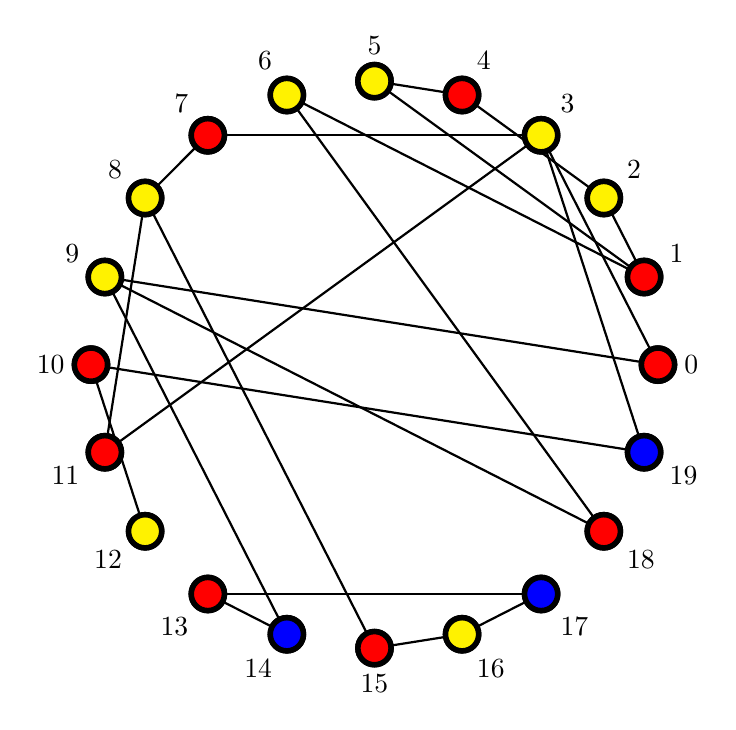
\begin{tikzpicture}[scale=1.2]
\renewcommand*{\VertexLineWidth}{2pt}
\GraphInit[vstyle=Welsh]
\Vertices[unit=3]{circle}{0,1,2,3,4,5,6,7,8,9,10,11,12,13,14,15,16,17,18,19}
\Edges(0,3)
\Edges(1,2)
\Edges(1,5)
\Edges(3,7)
\Edges(1,6)
\Edges(2,4)
\Edges(4,5)
\Edges(10,12)
\Edges(19,3)
\Edges(14,9)
\Edges(7,8)
\Edges(15,16)
\Edges(13,14)
\Edges(18,9)
\Edges(11,3)
\Edges(10,19)
\Edges(8,11)
\Edges(0,9)
\Edges(13,17)
\Edges(18,6)
\Edges(16,17)
\Edges(15,8)
\SetVertexNoLabel
\AddVertexColor{red}{0}
\AddVertexColor{red}{1}
\AddVertexColor{yellow}{2}
\AddVertexColor{yellow}{3}
\AddVertexColor{red}{4}
\AddVertexColor{yellow}{5}
\AddVertexColor{yellow}{6}
\AddVertexColor{red}{7}
\AddVertexColor{yellow}{8}
\AddVertexColor{yellow}{9}
\AddVertexColor{red}{10}
\AddVertexColor{red}{11}
\AddVertexColor{yellow}{12}
\AddVertexColor{red}{13}
\AddVertexColor{blue}{14}
\AddVertexColor{red}{15}
\AddVertexColor{yellow}{16}
\AddVertexColor{blue}{17}
\AddVertexColor{red}{18}
\AddVertexColor{blue}{19}
\end{tikzpicture}
\caption{TikZ-Graph generated in Sun Dec 27 02:14:58 2015
.}
\end{figure}
\vspace{0.5cm}
\begin{center}For more details: {\tt tolribeiro.github.com/repository}\end{center}.\end{document}
